%%%%%%%%%%%%%%%%%%%%%%%%%%%%%%%%%%%%%%%%%%%%%%%%%%%%%%%%%%%%%%%%%%%%%%%%%%%
%% This file is part of the book
%%
%% Algorithmic Graph Theory
%% http://code.google.com/p/graph-theory-algorithms-book/
%%
%% Copyright (C) 2009, 2010 Minh Van Nguyen <nguyenminh2@gmail.com>
%%
%% See the file COPYING for copying conditions.
%%%%%%%%%%%%%%%%%%%%%%%%%%%%%%%%%%%%%%%%%%%%%%%%%%%%%%%%%%%%%%%%%%%%%%%%%%%

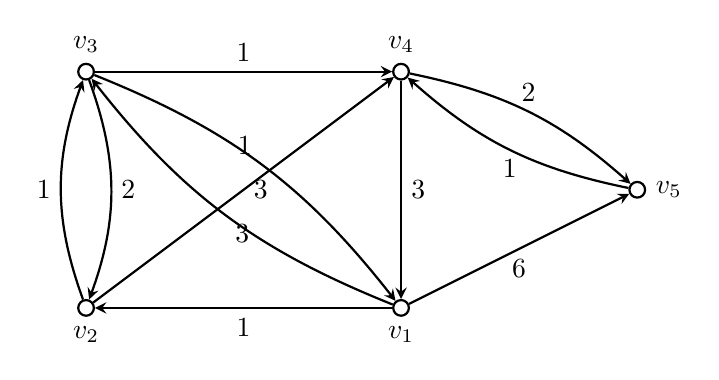
\begin{tikzpicture}
[nodedecorate/.style={shape=circle,inner sep=2pt,draw,thick},%
  arrowdecorate/.style={->,>=stealth,thick}]
%% nodes or vertices
\foreach \nodename/\x/\y/\direction/\navigate in {v_1/4/0/below/south,
  v_2/0/0/below/south, v_3/0/3/above/north, v_4/4/3/above/north,
  v_5/7/1.5/right/east}
{
  \node (\nodename) at (\x,\y) [nodedecorate] {};
  \node [\direction] at (\nodename.\navigate) {$\nodename$};
}
%% edges or lines
\path
\foreach \startnode/\endnode/\direction/\weight in {v_1/v_2/below/1,
  v_1/v_5/below/6, v_2/v_4/right/3, v_3/v_4/above/1, v_4/v_1/right/3}
{
  (\startnode) edge[arrowdecorate] node[\direction]{$\weight$} (\endnode)
}
\foreach \startnode/\endnode/\direction/\angle/\weight in {
  v_3/v_2/right/20/2, v_3/v_1/above left/15/1, v_2/v_3/left/20/1,
  v_1/v_3/below right/15/3, v_4/v_5/above/15/2, v_5/v_4/below/15/1}
{
  (\startnode) edge[arrowdecorate,bend left=\angle] node[\direction]{$\weight$} (\endnode)
};
\end{tikzpicture}
